\documentclass{article}
\usepackage[utf8]{inputenc}
\usepackage{graphicx}
\usepackage{tabularx}
\usepackage{geometry}
\geometry{a4paper, left=2.5cm, heightrounded}

\begin{document}
    \author{Domenico Vitale N86003234, Luca Rea N86003674} 
    \title{\LARGE Traccia 3: Sistema di gestione di una rubrica telefonica avanzata}
    \maketitle

    \begin{center}
    
\includegraphics[scale=0.15]{/home/luca/Documenti/Progetto basi dati/Latex/Foto.png}
    \end{center}

    \newpage
    \renewcommand\contentsname{Indice}
    \tableofcontents
    \newpage

    \section{\LARGE La traccia}
    Si sviluppi un sistema informativo, composto da una base di dati relazionale e da un applicativo Java dotato
    di GUI (Swing o JavaFX), per la gestione di una rubrica telefonica avanzata.
    \\La rubrica deve essere in grado di consentire la memorizzazione e visualizzazione di dati riguardanti contatti.
    Per ogni contatto la rubrica deve ricordare il nome e cognome della persona cui si riferisce. Inoltre, può essere
    eventualmente memorizzata anche una foto (della quale bisogna ricordare il percorso sul disco dove può
    essere reperita). \\I contatti possono essere organizzati in gruppi (dotati di un nome) che comprendono uno o più contatti.
    \\I gruppi possono anche intersecarsi tra loro, cosicché un contatto può anche appartenere a più di un gruppo.
    \\Per ogni contatto, bisogna mantenere un insieme (eventualmente vuoto) dei suoi indirizzi di posta
    elettronica. Inoltre, bisogna anche ricordare tutti gli account a sistemi di messaging. Per ognuno di questi
    account, bisogna ricordare il fornitore (ad esempio Whatsapp, Telegram, Teams, etc.), il nickname dichiarato
    dal contatto, la frase di benvenuto e l’indirizzo e-mail collegato a tale account. \\L’indirizzo e-mail deve essere
    necessariamente tra gli account di posta già salvati per il contatto.
    \\Per ogni contatto possono poi essere mantenuti suoi indirizzi fisici (per ognuno di essi, bisogna conoscere
    Via, Città, CAP, Nazione). In particolare, deve essere obbligatoriamente definito un indirizzo principale,
    mentre possono esserci uno o più eventuali altri indirizzi secondari.
    \\Infine, per ogni contatto devono essere mantenuti i suoi eventuali numeri telefonici, distinguendo tra telefoni
    fissi e mobili. Per ogni telefono mobile, può essere indicato un telefono fisso cui verranno reindirizzate
    eventuali chiamate senza risposta e, analogamente per ogni telefono fisso deve essere indicato un telefono
    mobile per il reindirizzamento. Ogni contatto deve avere almeno un telefono fisso e un telefono mobile.
    \\Si tenga conto che il sistema accetta contatti che dichiarino stessi indirizzi fisici o numeri telefonici ma non
    accetta contatti che dichiarano stesse e-mail.
    \\Il sistema deve fornire funzionalità per aggiungere nuovi contatti e creare, modificare o eliminare ognuna
    delle informazioni in esso contenute. Inoltre, devono essere realizzate funzionalità per la ricerca dei
    contatti per nome, per email, per account di messaging e per numero di telefono

    \section{\LARGE Class diagram}
    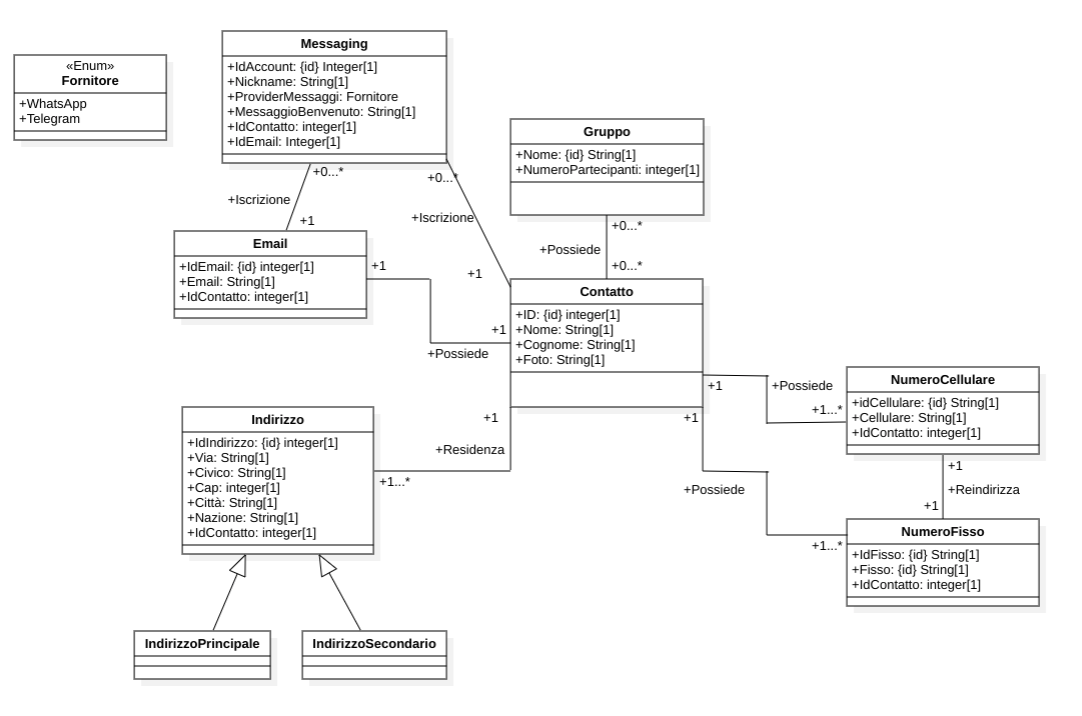
\includegraphics[scale=0.5]{/home/luca/Documenti/Progetto basi dati/Latex/Non_ristrutturato.png}
   

    \section{\LARGE Class diagram ristrutturato}
    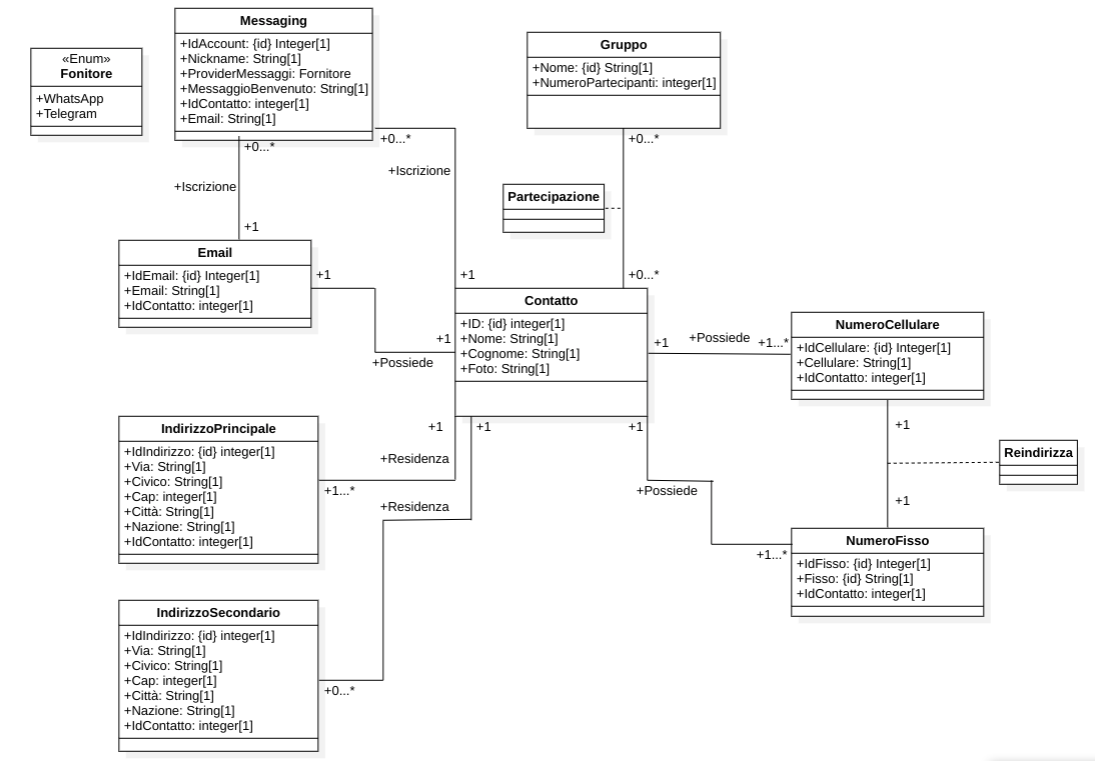
\includegraphics[scale=0.48]{/home/luca/Documenti/Progetto basi dati/Latex/Ristrutturato.png}


    \section{\LARGE Dizionario delle classi}
        \begin{tabular}{| m{3cm} | m{6cm}| m{6cm} |}
            \hline
            \textbf{CLASSE} &\textbf{DESCRIZIONE} & \textbf{ATTRIBUTI}\\
            \hline
            Contatto & Classe che contiene tutte le informazioni sul contatto &
            ID: codice univoco contatto\newline
            Nome: il nome del contatto\newline
            Cognome: il cognome del contatto\newline
            Foto: foto profilo del contatto\\
            \hline
            IndirizzoPrincipale & Classe che contiene le informazioni sull'indirizzo principale &
            IdIndirizzo: codice univoco indirizzo\newline
            Via\newline
            Civico\newline
            Cap\newline
            Città\newline
            Nazione\newline
            IdContatto: chiave esterna della classe contatto\newline\\
            \hline
            IndirizzoSecondario & Classe che contiene le informazioni sull'indirizzo secondario &
            IdIndirizzo: codice univoco indirizzo\newline
            Via\newline
            Civico\newline
            Cap\newline
            Città\newline
            Nazione\newline
            IdContatto: chiave esterna della classe contatto\newline\\
            \hline
            Email & Classe che contiene le informazioni sull' indirizzo email principale di un contatto &
            IdEmail: codice univoco email\newline
            Email\newline
            IdContatto: chiave esterna della classe contatto\\
            \hline
            NumeroCellulare & Classe che contiene il numero di cellulare del contatto &
            IdCellulare: codice univoco cellulare\newline
            NumeroCellulare\newline
            IdContatto: chiave esterna di contatto\\
            \hline
            NumeroFisso & Classe che contiene il numero di telefono fisso &
            IdFisso:  codice univoco fisso\newline
            NumeroFisso\newline
            IdContatto: chiave esterna di contatto\\
            \hline
            Messaging & Classe che contiene tutte le informazioni per le applicazioni di messaging &
            Nickname\newline
            Provider: nome del servizio di messaggistica\newline
            MessaggioBenevnuto: piccola frase di benvenuto\newline
            IdContatto\newline
            IdEmail\newline
            IdAccount: codice univoco di messaging\\
            \hline
            Gruppo & Classe che contiene informazioni sui gruppi &
            Nome: codice univoco di gruppo\newline
            NumeroPartecipanti: il numero di partecipanti al gruppo\\
            \hline
            Partecipazione & Classe che contiene informazioni sui contatti nei gruppi &
            IdContatto: chiave esterna di contatto\newline
            NomeGruppo: chiave esterna di gruppo\\
            \hline
    
        \end{tabular}

    \section{\LARGE Dizionario delle associazioni}
        \begin{tabular}{| m{3cm} | m{6cm}| m{6cm} |}
            \hline
            \textbf{ASSOCIAZIONE} &\textbf{DESCRIZIONE} & \textbf{PARTECIPANTI}\\
            \hline
            Partecipazione & Descrive il legame tra contatto e gruppo in quanto ogni contatto può partecipare in più gruppi e ogni gruppo può ospitare più contatti &
            IdContatto: è membro (0,n)\newline
            NomeGruppo: ospita (0,n)\\
            \hline
        \end{tabular}
    \\ \\ \\
    \section{\LARGE Dizionario dei vincoli}
    1)Il numero di telefono cellulare deve essere obbligatoriamente uguale a 10 cifre.\\
    2)Il numero di telefono fisso deve essere  obbligatoriamente compreso tra 9 e 11 cifre.\\
    3)Il cap deve essere obbligatoriamente uguale a 5 cifre.
    \section{\LARGE Schema logico}
    Contatto: (\textbf{ID}, Nome, Cognome, Foto);\\
    Email: (\textbf{IdEmail}, IdContatto, Email);\\
    Gruppo: (\textbf{Nome}, NumeroPartecipanti);\\
    Partecipazione: (IdContatto, NomeGruppo);\\
    NummeroCellulare: (\textbf{IdCellulare}, Cellulare, IdContatto);\\
    NumeroFisso: (\textbf{IdFisso}, Fisso,  IdContatto);\\
    Messaging: (\textbf{IdAccount}, Nickname, ProviderMessaggi, MessaggioBenvenuto, IdContatto, IdEmail);\\
    IndirizzoPrincipale: (\textbf{IdIndirizzo}, Via, Civico, Cap, Città, Nazione, IdContatto);\\
    IndirizzoSecondario: (\textbf{IdIndirizzo}, Via, Civico, Cap, Città, Nazione, IdContatto);

    \newpage
    \section{\LARGE Descrizione dei triggers}
    1)Il trigger "ControlloAppartenenzaGruppi" si attiva prima dell'esecuzione di un 
    inserimento nella tabella "Partecipazione" ed esegue la funzione "ControlloAppartenenzaGruppo()".\\
    2)Il trigger "PartecipantiRimuovi" si attiva dopo l'esecuzione di una cancellazione
    sulla tabella partecipazione ed esegue la funzione "RimuoviPartecipanti()".\\
    3)Il trigger "PartecipantiAggiungi" si attiva dopo l'esecuzione di un inserimento
    sulla tabella partecipazione ed esegue la funzione "AumentoPartecipanti()".\\
    4)Il trigger "RimuoviNumeroCellulare" si attiva prima dell'esecuzione di una cancellazione sulla tabella 
    contatto ed esegue la funzione "EliminaContatto()".\\
    5)Il trigger "EliminaMessaging" si attiva prima dell'esecuzione di una cancellazione sulla tabella email
    ed esegue la funzione "EliminaMessaging()".\\
    6)Il trigger "AggiornaEmailMessaging" si attiva dopo un aggiornamento sulla tabella email ed esegue la funzione
    "AggiornaEmailMessaging()".


    \section{\LARGE Descrizione functions}
    1)La funzione "RimuoviPartecipanti()" si occupa di decrementare il numero di partecipanti
    attivi nel gruppo.\\
    2)La funzione "AumentoPartecipanti()" si occupa di aumentare il numero di partecipanti
    attivi nel gruppo\\
    3)La funzione "ControlloAppartenenzaGruppo()" si occupa di controllare che non ci siano
    contatti duplicati presenti nel gruppo.\\
    4)La funzione "EliminaContatto()" si occupa di eliminare il contatto eliminando prima tutte 
    le dipendenze alle altre tabelle.\\
    5)La funzione "AggiornaEmailMessaging()" si occupa di aggiornare l'email degli account di messaggistica
    quando viene modificata nella tabella email.\\
    6)La funzione "EliminaMessaging()"  si occupa di eliminare la dipendenza dell'email dalla tabella
    messaging quando viene eliminata un'email principale. 

\end{document}